

% This is mymiccaipaper.tex the demonstration file of
% MICCAI 2006 for Latex2e
% adapted from LLNCS.DEM from
% the LaTeX macro package from Springer-Verlag
% for Lecture Notes in Computer Science,
% version 2.2 for LaTeX2e
%
%\documentclass[runningheads]{llncs}
\documentclass[a4paper, lmargin=1.925cm, rmargin=1.925cm,tmargin=2.54cm,bmargin=4.94cm]{spie}
%
\usepackage{makeidx}  % allows for indexgeneration
%st added this to help with anonymisation
%otherwise it took my name from one of the eps file
%This still got overwritten by the last eps file,
%had to manually pull the author out of that.
\pdfinfo{
%letterpaper,
%colorlinks,
%urlcolor=black,
pdfpagemode=none,
pdftitle={SciKit-SurgeryGlenoid},
pdfauthor={Stephen Thompson},
pdfcreator={},
pdfsubject={},
pdfkeywords={}
}
		  
%
\usepackage{multirow}
\usepackage{subcaption}
\usepackage{graphicx}
\usepackage{rotating}
\usepackage{array}
\usepackage{pifont}
\usepackage{url}
\usepackage{hyperref}

%this is trying to make a nice code listing box
\usepackage{listings}
\usepackage{xcolor}

\definecolor{codegreen}{rgb}{0,0.6,0}
\definecolor{codegray}{rgb}{0.5,0.5,0.5}
\definecolor{codepurple}{rgb}{0.58,0,0.82}
\definecolor{backcolour}{rgb}{0.95,0.95,0.92}

\lstdefinestyle{mystyle}{
    backgroundcolor=\color{backcolour},
    commentstyle=\color{codegreen},
    keywordstyle=\color{magenta},
    numberstyle=\tiny\color{codegray},
    stringstyle=\color{codepurple},
    basicstyle=\ttfamily\footnotesize,
    breakatwhitespace=false,
    breaklines=true,
    captionpos=b,
    keepspaces=true,
    numbers=left,
    numbersep=5pt,
    showspaces=false,
    showstringspaces=false,
    showtabs=false,
    tabsize=2,
    xleftmargin=4.0ex
}

\lstset{style=mystyle}


\graphicspath{{pics/}{figs/}}
% list here all the paths to your figure folders
\usepackage{glossaries} %st - put this in to deal with acronyms tidily
%\usepackage[acronym=true,description]{glossaries} %st - put this in to deal with acronyms tidily
\glsdisablehyper 
 %removed relative path and replaced with symbolic link in this directory, see makefile.

\newcommand{\sksurgery}{SciKit-Surgery }
\newcommand{\sksglenoid}{SciKit-SurgeryGlenoid }
\newcommand{\sksglenoidns}{SciKit-SurgeryGlenoid}
\newcommand{\core}{SciKit-SurgeryCore }
\begin{document}
%
%\frontmatter          % for the preliminaries
%
%\authorrunning{S. Thompson et al.}   % abbreviated author list (for running head)
%\pagestyle{headings}  % switches on printing of running heads
%\pagestyle{empty}  % switches off printing of running heads
\pagestyle{plain}
%
%\mainmatter              % start of your contributions
%
\title{SciKit-SurgeryGlenoid, an Open Source Toolkit for Glenoid Version Measurement}
%\titlerunning{SciKit-SurgeryGlenoid}  % abbreviated title (for running head)
%
\author{Asta~Olafsdottir\supit{1}, Addie~Majed\supit{2}, David~Butt\supit{2}, Mark~Falworth\supit{2},
Stephen~Thompson\supit{1}
\skiplinehalf
\supit{1}Wellcome/EPSRC Centre for Interventional and Surgical Science, University College London, United Kingdom \\
\supit{2}The Royal National Orthopaedic Hospital NHS Trust\\
}

\maketitle              % typeset the title of the contribution

\begin{abstract}
%https://spie.org/MI22/conferencedetails/image-guided-procedures?enableBackToBrowse=true

Correct understanding of the geometry of the glenoid (the socket of the shoulder joint) is 
key to successful planning of shoulder replacement surgery. This surgery typically involves 
placing an implant in the shoulder joint to restore joint function. The most relevant 
geometry is the glenoid version, which is the angular orientation of the glenoid surface 
relative to the long axis of the scapula in the axial plane. However, measuring the glenoid version is not 
straightforward and there are multiple measurement methods in the literature and used in 
commercial planning software. 

In this paper we introduce SciKit-SurgeryGlenoid, an open source toolkit for the measurement
of Glenoid version. SciKit-SurgeryGlenoid contains implementations of the 4 most    
frequently used glenoid version measurement algorithms enabling easy and unbiased comparison of
the different techniques. We present the results of using the software on 10(?) sets of
pre-operative CT scans taken from patients who have subsequently undergone shoulder replacement surgery.

Here we describe the software and present results based on manual segmentation of 10
patients. We further compare these results with those obtained from a commercial
implant planning software.



SciKit-SurgeryGlenoid currently requires manual segmentation of the relevant anatomical 
features for each method. Future work will look at automating the segmentation process
 to build an automatic and repeatable 
pipeline from {CT} or radiograph to quantitative glenoid version measurement.

\end{abstract}

\section{Introduction}
\label{sec:introduction}
Correct understanding of the geometry of the glenoid (the dish of the shoulder joint) is
key to successful planning of shoulder arthroplasty. This surgery typically involves
placing an implant in the shoulder joint to restore joint function. The most relevant
geometry is the glenoid version, which is the angular orientation of the glenoid surface
relative to the long axis of the scapula. However, measuring the glenoid version is not
straightforward and there are multiple measurement methods in the literature and used in
commercial planning software. Several papers look at the effect of using 
different methods for measuring glenoid version and propose their own 
methods, \cite{PMID:33330245, PMID:32010231, PMID:29298261, PMID:33554174}. 
Different approaches are also implemented by implant vendors and commercial 
software suppliers \cite{blueprint, exactech, djosurgical} however these methods can 
be somewhat opaque. 

\section{Methods}
\label{sec:methods}

\section{Results}
\label{sec:results}
\begin{table}
	\begin{center}
		\begin{tabular}{|p{0.2\linewidth}|p{0.2\linewidth}|p{0.2\linewidth}|} \hline
			Method & Mean Version & Standard Deviation \\ \hline
			Two Planes & 8.9\degree & 4.7\degree \\
			Corrected Friedman & 8.4\degree & 6.5\degree \\
			Friedman & 9.4\degree & 7.4\degree \\
			Vault & 12.3\degree & 7.7\degree \\
			Commercial software & 9.9\degree & 6.1\degree \\
                        \hline
		\end{tabular}
	\end{center}
	\caption{\label{tab:results}A comparison of the results of each method tested 
	on 10 retrospective patients}
\end{table}

Table \ref{tab:results} presents the results of using \sksglenoid on 10 patients.
The version measured using the planes method has a mean glenoid
version of 8.9\degree (SD, 4.7\degree; range, 5\degree to 20.9\degree), 
while mean glenoid version 
for the 3D corrected Friedman method 
was 8.4\degree (SD, 6.5\degree; range, -4.0\degree to 16.9\degree). 
For the 2D methods, the mean glenoid version for the 
Friedman method was 9.4\degree (SD, 7.4\degree; range, -0.7\degree to 24\degree) 
and for the vault model was 12.3\degree (SD, 7.7\degree; range, 4\degree to 26\degree).
In this 
case a positive value indicates retroversion while a negative value indicates anteversion of the 
glenoid. Overall, the 3D methods resulted in both lower mean version values as well as lower
variability, while the 2D methods revealed a slightly higher variability.

The measurements using these methods were also compared with version measurements on the same
10 patients using a commercial software\cite{djosurgical}. 
The planes method (r = 0.90, p = 0.0004), 
corrected Friedman method (r = 0.83, p = 0.0034), 
and conventional Friedman method (r = 0.79, p = 0.0064) 
all showed significant correlation with the commercial software. 
The vault method did not show significant correlation (r = 0.59, p = 0.074).  
The mean difference between the methods were overall not significant (p > 0.05), 
except for the vault method (p = 0.03). Correlation plots are shown in Figure \ref{fig:correl}.

\begin{figure}
	\begin{center}
		\begin{subfigure}[b]{0.30\linewidth}
			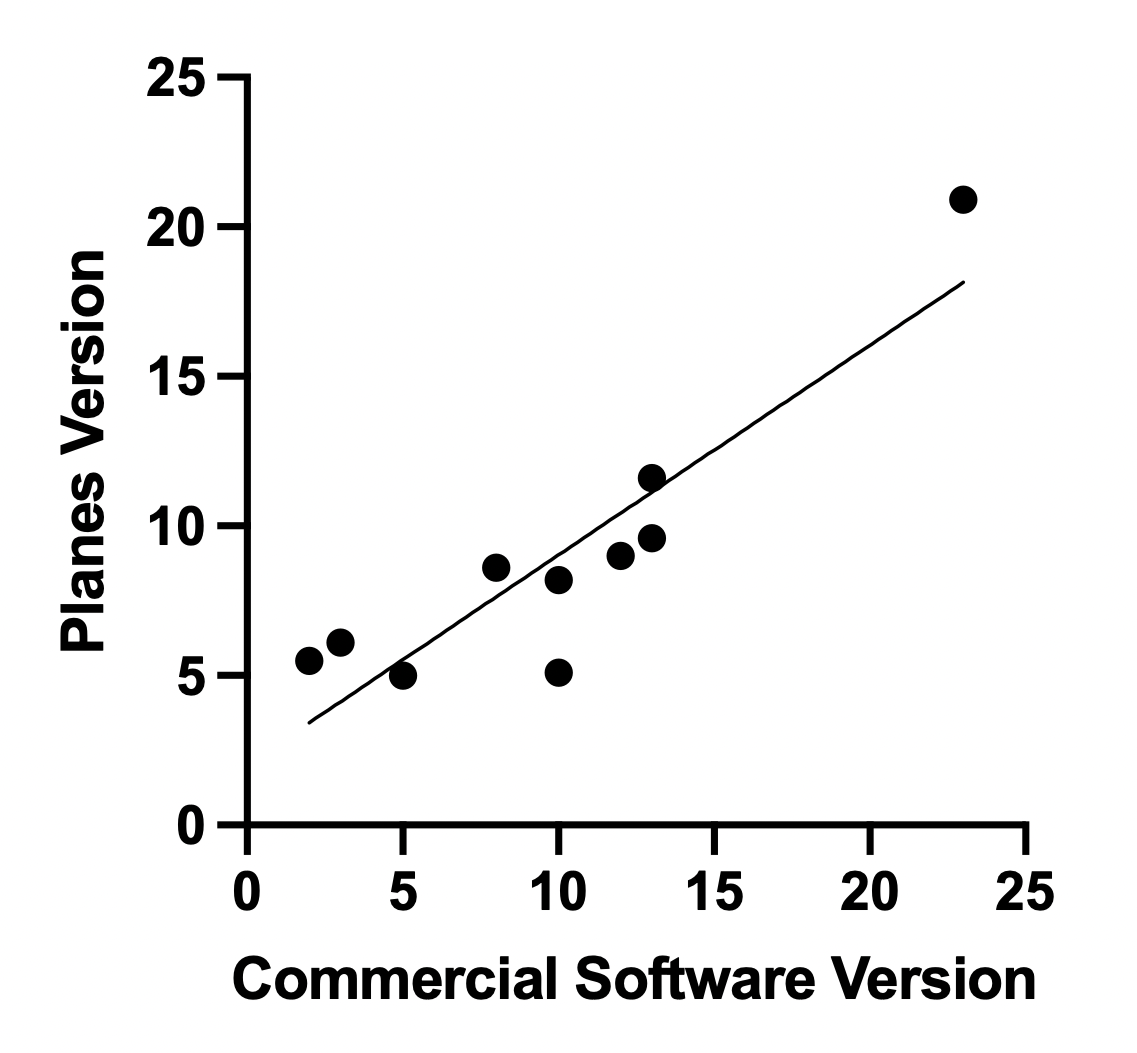
\includegraphics[width=\linewidth]{figures/planes.png}
			\caption{Two Planes Method}
		\end{subfigure}
		\begin{subfigure}[b]{0.30\linewidth}
			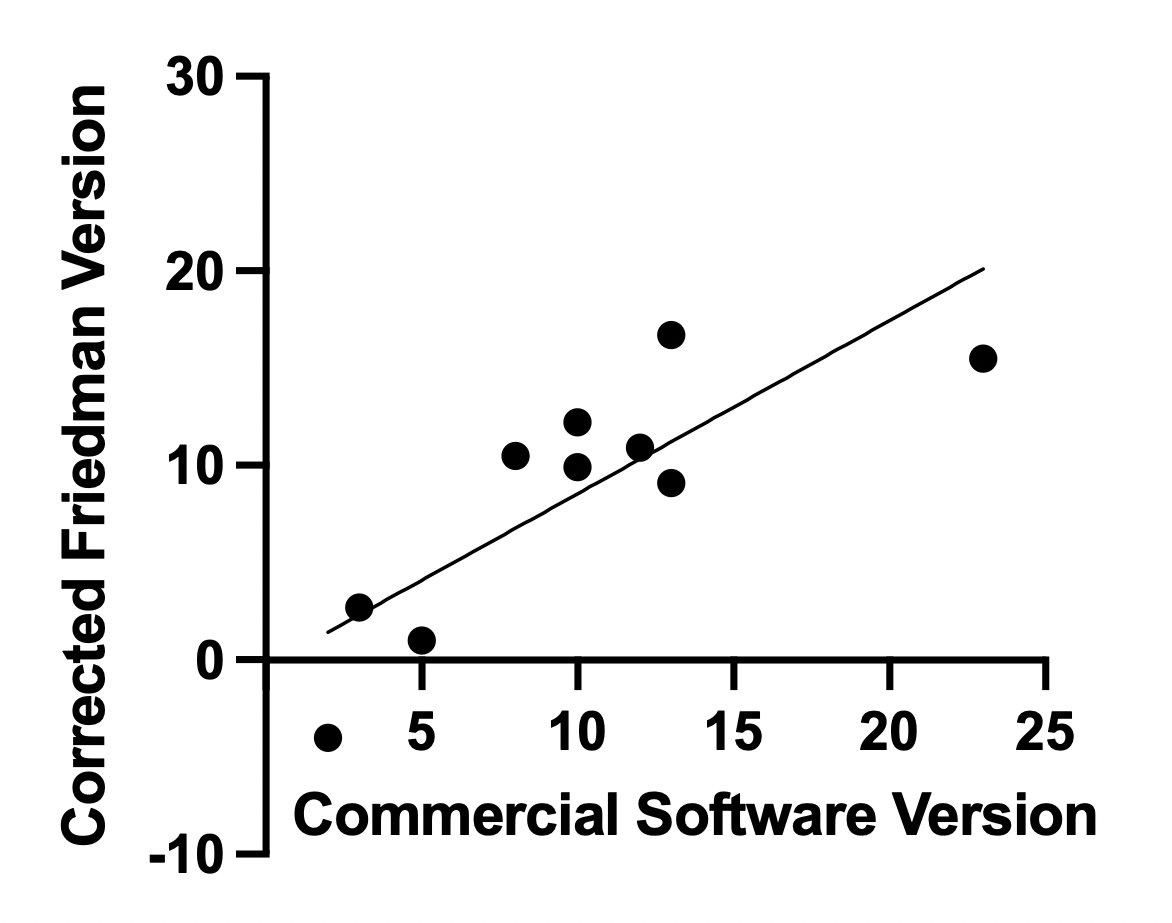
\includegraphics[width=\linewidth]{figures/correctedfried.png}
			\caption{Corrected Friedman Method}
		\end{subfigure}
		\begin{subfigure}[b]{0.30\linewidth}
			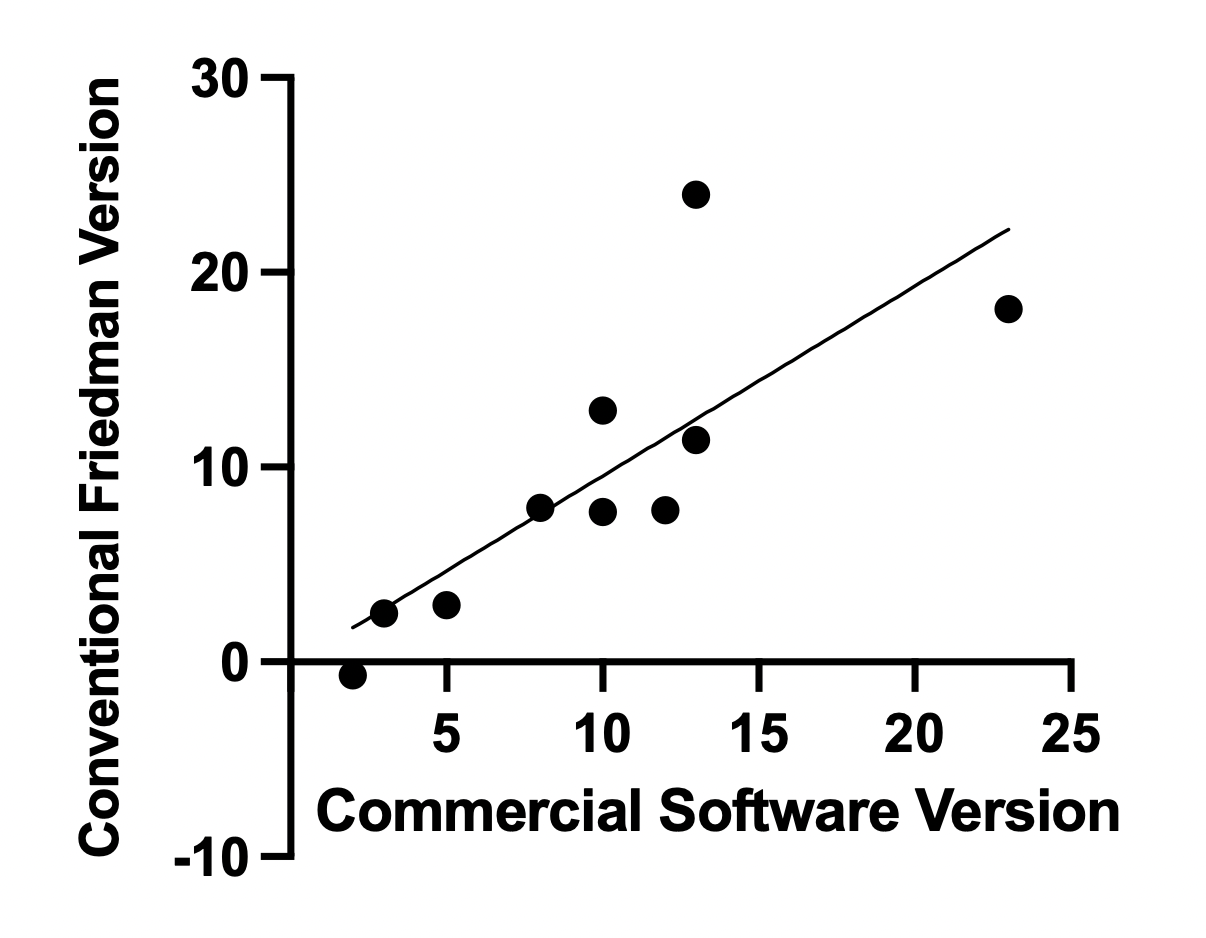
\includegraphics[width=\linewidth]{figures/friedman.png}
			\caption{Friedman Method}
		\end{subfigure}
		\caption{\label{fig:correl}The Pearson correlation between the commercial software and 3 of the methods. All show significant correlation.}
	\end{center}
\end{figure}

\section{Discussion}
\label{sec:discussion}
There are several methods that have been proven to be accurate in preoperative measurement of 
the glenoid version. Specifically, 3D methods have become the standard as they
provide a higher accuracy accounting for the positional errors during image acquisition
(Budge et al. \cite{BUDGE2011577}, Moineau et al. \cite{PMID:22964089}). 
Testing the most common 2D and 3D methods using the 
\sksglenoid toolkit allowed for an evaluation of its effectiveness in comparing these methods. 
The early results presented are consistent with 
previously reported results (Matsumura et al. \cite{PMID:24618285}, 
Budge et al. \cite{BUDGE2011577}, Ganapathi et al. \cite{PMID:20933439}).

While the mean version did not show any significant difference between most methods, 
this could be due to the small sample size used in this case. However, it is notable
that the 3D methods reveal slightly lower version means and lower standard deviations
which could prove significant when more scans are analysed with additional observers.

From the Pearson correlation coefficient, significant correlation between the commercial 
software and 3 out of the 4 methods was seen. The vault method showing little correlation
with the commercial software could be due to its much higher mean version value.
The vault method tends to overestimate the glenoid version as has been previously
reported by several studies (Cunningham et al. \cite{PMID:29778592},
Matsumura et al. \cite{PMID:24618285}). 
The correlation
tests prove however that there is good agreement between \sksglenoid and the
commercial software already in use, indicating accuracy and credibility of this toolkit.
While this can good indicator of reliability, further measurements using this software
by different observers would be needed to be able to test inter and intra observer reliability.
However, \sksglenoid proves to be promising in providing an unbiased way of
comparing the many different methods available to measure glenoid version.

Limitations of this initial testing of \sksglenoid include the small sample size used.
A study 
with a wider range of CT scans could reveal better understanding of the software’s reliability. 
Additionally, as points for each method were selected manually, there are some inaccuracies that 
arise which could be better understood with repeated measurements and multiple observers.

\section{Conclusion}
\sksglenoid provides a useful resource for shoulder arthroplasty. Future work could look at either 
automating the segmentation process using state of the art registration algorithms \cite{Fu2020} to create a fully automatic pipeline, or at integrating the library with 3DSlicer to create a 
``slicelet" based application, similar to our previous work \cite{PMID:33937966} in skull base 
navigation.


\section{Other Submissions}
This work has not been submitted for publication or presentation elsewhere.

\section{Open Access and Open Data}
This research was funded in whole, or in part, by the Wellcome Trust [203145Z/16/Z]. 
For the purpose of Open Access, the author has applied a CC BY public copyright licence to any Author Accepted Manuscript version arising from this submission.
The data described in Sections \ref{sec:methods} and \ref{sec:results} was collected under
research ethics application XXXXX ? and if permitted will be made freely available alongside
this publication. 

\section{Acknowledgements}
This work is supported by the Wellcome/EPSRC Centre for Interventional and Surgical Sciences (WEISS) [203145Z/16/Z].



%\bibliographystyle{spie2008/myspiebib}
\bibliographystyle{spmpsci}

\bibliography{surgeryglenoid-paper.bib}

\end{document}
